% status: 0
% chapter: TBD

\title{Universal Cloud REST Service Framework to Determine 
the Validity Of Benford’s Law Using Datasets In Data.gov}

\author{Ravinder Lambadi}
\affiliation{%
  \department{School of Informatics, Computing, and Engineering}
  \institution{Indiana University}
  \city{Bloomington}
  \state{IN}
  \postcode{47408}
  \country{USA}}
\email{rlambadi@iu.edu}


\author{Orly Esteban}
\affiliation{%
  \department{School of Informatics, Computing, and Engineering}
  \institution{Indiana University}
  \city{Bloomington}
  \state{IN}
  \postcode{47408}
  \country{USA}}
\email{esteban@iu.edu}

\begin{abstract}
It is observed that a lot of real-life data, from personal 
expenses to world population data, tend to obey Benford’s Law. 
Because of this phenomenon, Benford’s Law has been leveraged 
in a lot of statistical analysis – including fraud detection. 
In 2009,  Benford’s Law has been utilized to detect election 
fraud in Iran. In this paper, the authors will determine the 
universality of the law. Is the law applicable to any dataset? 
The authors will analyze and visualize data on publicly available 
data sets at data.gov and determine which datasets follow this 
law and which ones do not, if any.
\end{abstract}

\keywords{hid-sp18-514, hid-sp18-506, REST, Benford's Law, Python}

\maketitle

\section{Introduction}
Benford’s law is a phenomenon about the distribution of 
the first-digits of numerical sets of real-life data. 
The law states that the distribution of the first digits 
follows a certain mathematical pattern. For example, the 
digit 1 tends to occur about 30 percentage of the time compared 
to 11 percentage if the distribution is evenly flat. 
The probability distribution tends to go lower from the 
digit 1 to the digit 9 ~\cite{hid-sp18-514-benfordwiki}.

A dataset is said to satisfy Benfords Law if the leading 
digits have the following the probability distribution: 

\begin{figure}[!ht]
\centering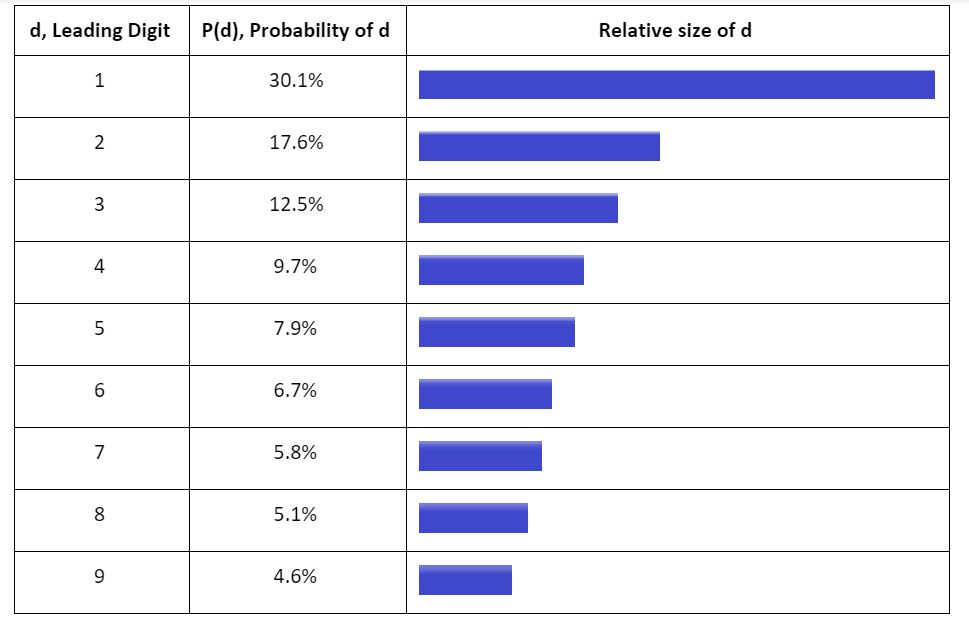
\includegraphics[width=\columnwidth]{images/benfords_law.JPG}
  \caption{Probability distribution of Benfords Law}\label{f:probability-dist-benfordlaw}
\end{figure}


In mathematical terms, Benford’s Law can be represented 
by the following equation:

P(d) = log (d+1) - log (d)

Example: In case base 10 is used we obtain the 
probability for the leading digit 1, as

P(1) = log (1+1) - log(1) = 0.301

which means, if the dataset complies 
with Benford's Law, the probability of finding a 
leading digit 1 is about 30.1 percentage of the time. 
Therefore, Benford’s Law indicates that the most 
likely leading digit for us to see is 1, the second 
most likely 2, the third most 3, the fourth most 
likely 4, and so on.

The logarithmic function can be in any base. We will 
be developing a REST service that allows the 
calculation of Benfords Law. The service will allow 
us to specify the base and the data set as input.

Benford’s law not only applys to the scale invariant 
data but also applies to various data sources, 
that we are going to analyze and visualize in this project.


\section{REST Services To Determive Benfords's Law}

There are two universal services have been built to determine
whether the provided data set follows Befords's law.

\begin{enumerate}
 \item BenfordLawExcelDataSetService
 \item BenfordLawCSVDataSetService
\end{enumerate}

\subsection{BenfordLawExcelDataSetService}
BenfordLawExcelDataSetService is a REST API service tested on 
on-premise and cloud environment. This service requires three 
input paramaters to determine Befords's Law. This service
downloads, process and send back the output 
for all excel based datasets.

Below parameters need to pass to this REST API:

\begin{enumerate}
\item dataLocation - Location of the dataset. 
 Ex: ~\cite{hid-sp18-514-excelDatalocation}
\item columnName - Name of the column in the 
 dataset for which Benford Law determation required. 
 Ex: Price
\item fileName - Dataset file name to be downloaded 
 as, Ex: nsn-extract.xlsx
\end{enumerate}

\subsection{BenfordLawCSVDataSetService}
BenfordLawCSVDataSetService is a REST API service 
tested on on premise and cloud environment. 
This service requires three input paramaters to 
determine Befords's Law. This service
downloads, process and send back the output 
for all CSV and Text based datasets .

Below parameters need to pass to this REST API:

\begin{enumerate}
\item dataLocation - Location of the dataset. 
 Ex: ~\cite{hid-sp18-514-csvDatalocation}
\item columnName - Name of the column in the 
 dataset for which Benford Law determation required. 
 Ex: COUNT PUBLIC ASSISTANCE TOTAL
\item fileName - Dataset file name to be downloaded 
 as,Ex: DemographicStatistics.csv
\end{enumerate}

\subsection{Benfords Law Verification for National Stock 
Number Extract Datset - Excel}
National Stock Number extract includes the current 
listing of National Stock Numbers (NSNs) , 
NSN item name and descriptions, and current 
selling price of each product listed in GSA 
Advantage and managed by GSA. Each NSN is 
listed with the vendors description of the item. 
Some descriptions exceed the standard length and are 
truncated ~\cite{hid-sp18-514-nsn-ds-desc}.

BenfordLawExcelDataSetService returned the below
output for the dataset ~\cite{hid-sp18-514-excelDatalocation}
and columns name was : Price.

\begin{figure}[!ht]
\centering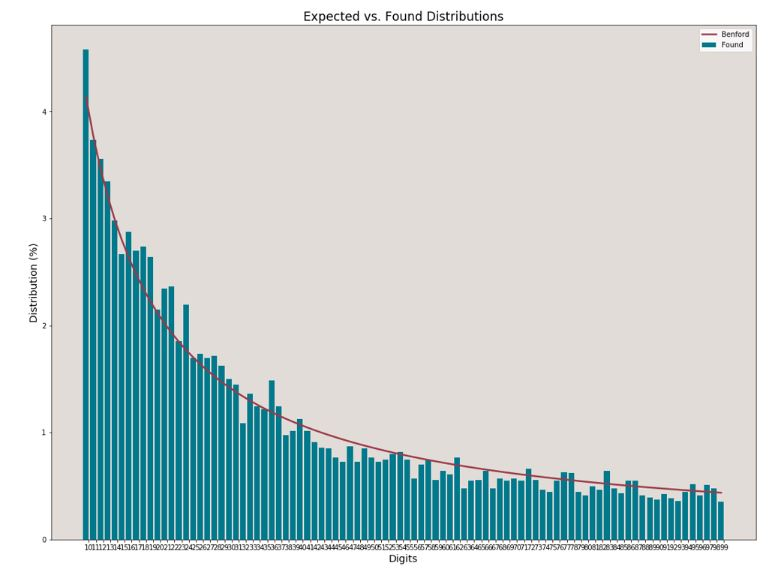
\includegraphics[width=\columnwidth]{images/benford_nsn.JPG}
  \caption{Benfords Law Verification for - NSN DS}\label{f:NSN-ds-benfordlaw}
\end{figure}

The line is Benford’s Law probabilities and the bars are 
the actual occurrences.


\subsection{Fraud Detection - Credit card transactions Dataset}
This dataset contains information on purchases made through 
the purchase card programs administered by the state and higher 
ed institutions. The purchase card information will be updated monthly 
after the end of the month. For example, July information will 
be added in August ~\cite{hid-sp18-514-purchase-card-desc}

BenfordLawCSVDataSetService returned the below
output for the dataset ~\cite{hid-sp18-514-purchase-card-ds}

\begin{figure}[!ht]
\centering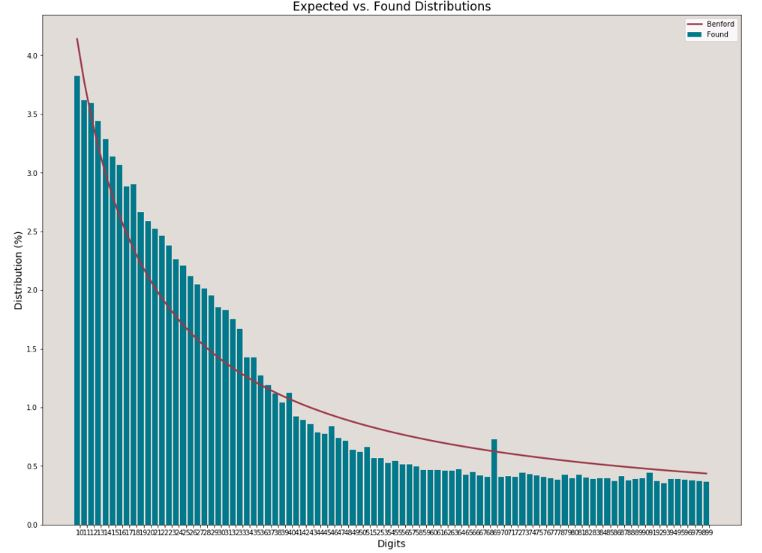
\includegraphics[width=\columnwidth]{images/benford_card_transactions.JPG}
  \caption{Fraud Detection Using Benford Law}\label{f:card-ds-benfordlaw}
\end{figure}

The line is Benford’s Law probabilities and the bars are 
the actual occurrences.


\section {Conclusion}
Benford’s Law can recognize the probabilities of highly 
likely or highly unlikely frequencies of numbers in a data set.
The probabilities are based on mathematical logarithms of 
the occurrence of digits from the given data sets for Benfords 
validity. We have verified Benford law for
stock price dataset and fraud detection on card transactions.
The limitation with Benford Law is, it performs Benford Law
analysis on Numeric data type column only. And for occurate
analysis it requires large dataset. For smaller dataset 
the analysis might not accurate.

\bibliographystyle{ACM-Reference-Format}
\bibliography{report} 
